\documentclass{article}

\usepackage{pandekten}

\usepackage{dashrule}

\makeatletter
\newcommand*{\shifttext}[1]{%
  \settowidth{\@tempdima}{#1}%
  \hspace{-\@tempdima}#1%
}
\newcommand{\plabel}[1]{%
\shifttext{\textbf{#1}\quad}%
}
\newcommand{\prule}{%
\begin{center}%
\hdashrule[0.5ex]{.99\linewidth}{1pt}{1pt 2.5pt}%
\end{center}%
}

\makeatother

\setlength{\parindent}{0pt}

\title{Assignment 1}
\author{Ze Chen}

\begin{document}

\maketitle

\plabel{1 (a)}%
The 5 lowest lying states are given below.
\begin{center}
    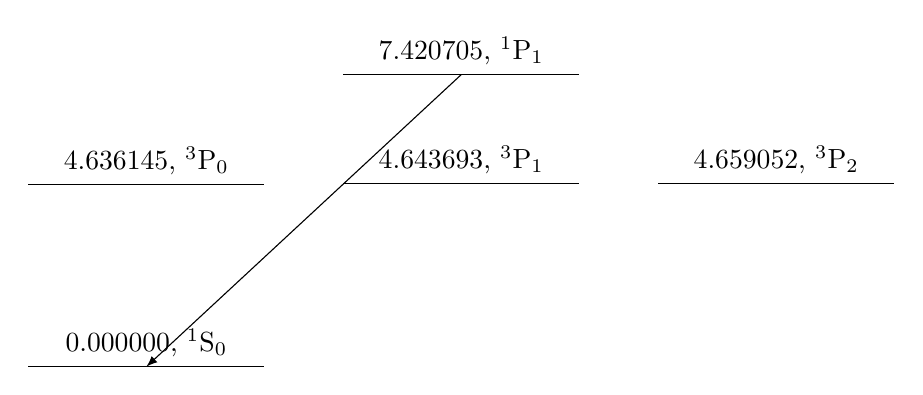
\begin{tikzpicture}[yscale=0.5]
        \draw[] (0, 0) -- (3, 0) node[midway,above]{\SI{0.000000}{\eV}, $\mathrm{^1S_0}$};
        \draw[] (0, 4.636145) -- (3, 4.636145) node[midway,above] {\SI{4.636145}{\eV}, $\mathrm{^3P_0}$};
        \draw[] (4, 4.643693) -- (7, 4.643693) node[midway, above]{\SI{4.643693}{\eV}, $\mathrm{^3P_1}$};
        \draw[] (8, 4.659052) -- (11, 4.659052) node[midway,above]{\SI{4.659052}{\eV}, $\mathrm{^3P_2}$};
        \draw[] (4, 7.420705) -- (7, 7.420705) node[midway,above]{\SI{7.420705}{\eV}, $\mathrm{^1P_1}$};
        %
        \draw[-latex] (5.5, 7.420705) -- (1.5, 0);
        %\draw[-latex] (5.5, 4.643693) to[out=-110,in=-70] (1.5, 4.636145);
        %\draw[-latex] (9.5, 4.659052) to[out=-110,in=-70] (5.5, 4.643693);
    \end{tikzpicture}
\end{center}

\plabel{(b)}%
The selection rule is given by
\begin{align*}
    \Delta J &= \qty{0,\pm 1}, \\
    \Delta M_J &= \qty{0, \pm 1}, \\
    \Delta S &= 0, \\
    \Delta L &= \qty{0,\pm 1}, \\
    \text{but no } L &= 0 \rightarrow L = 0 \text{ transitions}, \\
    \text{Laporte rule } (-1)^{\Delta \sum_i l_i} &\neq 1.
\end{align*}

\plabel{(c)}%
The only stable isotope is \ce{^{27}Al}, where $I=5/2$.
The F-levels are given below.
\begin{center}
    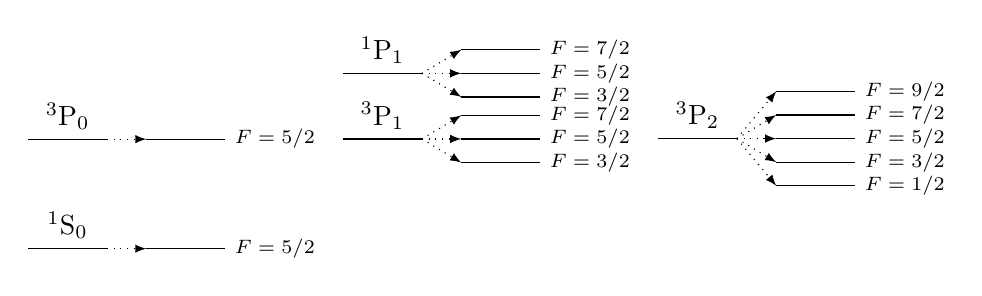
\begin{tikzpicture}[yscale=0.3]
        \draw[] (0, 0) -- (1, 0) node[midway,above]{$\mathrm{^1S_0}$};
        \draw[dotted,-latex] (1,0) --++(0.5,0);
        \draw (1,0) ++(0.5,0) --++(1,0) node[right] {\scriptsize $F=5/2$};
        %
        \draw[] (0, 4.636145) -- (1, 4.636145) node[midway,above] {$\mathrm{^3P_0}$};
        \draw[dotted,-latex] (1,4.636145) --++(0.5,0);
        \draw (1,4.636145) ++(0.5,0) --++(1,0) node[right] {\scriptsize $F=5/2$};
        %
        \draw[] (4, 4.643693) -- (5, 4.643693) node[midway, above]{$\mathrm{^3P_1}$};
        \draw[dotted,-latex] (5,4.643693) --++(0.5,0);
        \draw[dotted,-latex] (5,4.643693) --++(0.5,1);
        \draw[dotted,-latex] (5,4.643693) --++(0.5,-1);
        \draw (5,4.643693) ++(0.5,0) --++(1,0) node[right] {\scriptsize $F=5/2$};
        \draw (5,4.643693) ++(0.5,1) --++(1,0) node[right] {\scriptsize $F=7/2$};
        \draw (5,4.643693) ++(0.5,-1) --++(1,0) node[right] {\scriptsize $F=3/2$};
        %
        \draw[] (8, 4.659052) -- (9, 4.659052) node[midway,above]{$\mathrm{^3P_2}$};
        \draw[dotted,-latex] (9,4.659052) --++(0.5,0);
        \draw[dotted,-latex] (9,4.659052) --++(0.5,1);
        \draw[dotted,-latex] (9,4.659052) --++(0.5,-1);
        \draw[dotted,-latex] (9,4.659052) --++(0.5,2);
        \draw[dotted,-latex] (9,4.659052) --++(0.5,-2);
        \draw (9,4.659052) ++(0.5,0) --++(1,0) node[right] {\scriptsize $F=5/2$};
        \draw (9,4.659052) ++(0.5,1) --++(1,0) node[right] {\scriptsize $F=7/2$};
        \draw (9,4.659052) ++(0.5,-1) --++(1,0) node[right] {\scriptsize $F=3/2$};
        \draw (9,4.659052) ++(0.5,2) --++(1,0) node[right] {\scriptsize $F=9/2$};
        \draw (9,4.659052) ++(0.5,-2) --++(1,0) node[right] {\scriptsize $F=1/2$};
        %
        \draw[] (4, 7.420705) -- (5, 7.420705) node[midway,above]{$\mathrm{^1P_1}$};
        \draw[dotted,-latex] (5,7.420705) --++(0.5,0);
        \draw[dotted,-latex] (5,7.420705) --++(0.5,1);
        \draw[dotted,-latex] (5,7.420705) --++(0.5,-1);
        \draw (5,7.420705) ++(0.5,0) --++(1,0) node[right] {\scriptsize $F=5/2$};
        \draw (5,7.420705) ++(0.5,1) --++(1,0) node[right] {\scriptsize $F=7/2$};
        \draw (5,7.420705) ++(0.5,-1) --++(1,0) node[right] {\scriptsize $F=3/2$};
    \end{tikzpicture}
\end{center}

\prule

\plabel{2 (a)}%
With $\vb{B} = B \hat{\vb{z}}$, the Hamiltonian in matrix form with basis
\[ \qty(\ket{m_J=+\frac{1}{2}},\ket{m_J=-\frac{1}{2}}) \otimes \qty(\ket{m_I=+\frac{1}{2}},\ket{m_I=-\frac{1}{2}}) \]
is given by
\begin{gather*}
    H = g \mu_{\mathrm{B}} B \frac{1}{2} \sigma_z \otimes \sigma_0 + g_{\mathrm{n}} \mu_{\mathrm{N}} B \frac{1}{2} \sigma_0 \otimes \sigma_z + A \frac{1}{4} \sum_{i=x,y,z} \sigma_i\otimes \sigma_i \\
    = \arraycolsep=-17pt \begin{pmatrix}
        \frac{1}{4} A + \frac{1}{2} g\mu_{\mathrm{B}} B + \frac{1}{2} g_{\mathrm{n}} \mu_{\mathrm{N}} B & & & \\
        & -\frac{1}{4} A + \frac{1}{2} g\mu_{\mathrm{B}} B - \frac{1}{2} g_{\mathrm{n}} \mu_{\mathrm{N}} B & \frac{1}{2} A \\
        & \frac{1}{2} A & -\frac{1}{4} A - \frac{1}{2} g\mu_{\mathrm{B}} B + \frac{1}{2} g_{\mathrm{n}} \mu_{\mathrm{N}} B \\
        & & & \frac{1}{4} A - \frac{1}{2} g\mu_{\mathrm{B}} B - \frac{1}{2} g_{\mathrm{n}} \mu_{\mathrm{N}} B
    \end{pmatrix}.
\end{gather*}

\plabel{(b)}%
The first two coefficients are given by
\[ g\mu_{\mathrm{B}} = 2.002 \times \mu_{\mathrm{B}} = h\times \SI{28.02}{\giga\hertz\per\tesla}, \]
and
\[ g_{\mathrm{n}} \mu_{\mathrm{N}} = 0.4923 \times \mu_{\mathrm{N}} = h \times \SI{3.753e-3}{\giga\hertz\per\tesla}. \]

\plabel{(c)}%
The plot is given below.
\begin{center}
    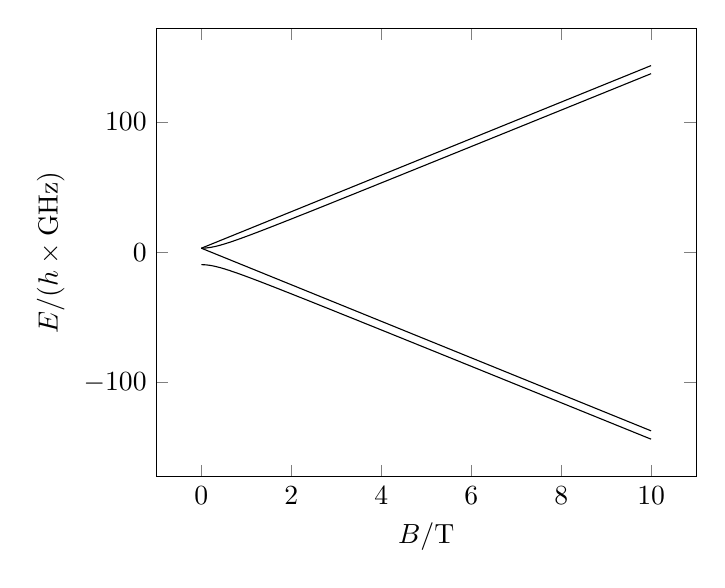
\begin{tikzpicture}
        \begin{axis}[domain=0:10,samples=100,xlabel=$B/\mathrm{T}$,ylabel=$E/(h\times \mathrm{GHz})$]
            \addplot[] {3.15 - 14.0119*x};
            \addplot[] {0.5*(-6.3 - sqrt(158.76 + 784.91 * x^2))};
            \addplot[] {3.15 + 14.0119*x};
            \addplot[] {0.5*(-6.3 + sqrt(158.76 + 784.91 * x^2))};
        \end{axis}
    \end{tikzpicture}
\end{center}

\plabel{(d)}%
The space generated by
\[ \qty{\ket{F=0,F_z=0}, \ket{F=1,F_z=0}} \]
has relative energy shift $\delta \Delta E = \bigO(B^2)$, where
\begin{align*}
    \Delta E &= \sqrt{A^2 + B^2(g \mu_{\mathrm{B}} - g_{\mathrm{n}} \mu_{\mathrm{N}})^2} \\
    &\approx A + \frac{(g \mu_{\mathrm{B}} - g_{\mathrm{n}} \mu_{\mathrm{N}})^2}{2A} B^2
\end{align*}
where
\[ \frac{(g \mu_{\mathrm{B}} - g_{\mathrm{n}} \mu_{\mathrm{N}})^2}{2A} = h\times \SI{31.15}{\giga\hertz\per\square\tesla}. \]

% \bibliographystyle{plain}
% \bibliography{main}

\end{document}
